\section{Конструкторская часть}

В данном разделе формулируются требования к программному обеспечению, описывается общая структура программы и детально рассматриваются алгоритмы, лежащие в основе визуализации и моделирования кинематики.

\subsection{Требования к программному обеспечению}

Разрабатываемое программное обеспечение предназначено для моделирования и визуализации работы шестереночных механизмов. К программе предъявляются следующие функциональные требования:
\begin{enumerate}
	\item программа должна предоставлять графический интерфейс пользователя для взаимодействия со сценой;
	\item должна быть реализована возможность добавления шестеренок различных размеров на гексагональную сетку;
	\item должна быть предусмотрена возможность удаления установленных шестеренок;
	\item программа должна обеспечивать визуализацию трехмерной сцены, включающей пол, сетку, оси и вращающиеся шестерни;
	\item должна быть реализована возможность управления камерой (вращение вокруг центра сцены, масштабирование);
	\item программа должна моделировать кинематику механизма: передачу вращения от ведущей шестерни к ведомым с учетом передаточных чисел;
	\item должен быть реализован контроль коллизий: запрет установки шестеренок в пересекающиеся позиции;
	\item должна быть предусмотрена индикация заклинивания механизма при создании противоречивых кинематических связей;
	\item программа должна позволять управлять скоростью и направлением вращения ведущей шестерни.
\end{enumerate}

\subsection{Разработка алгоритмов}

Для реализации поставленных задач были разработаны алгоритмы визуализации и расчета физики сцены.

\subsubsection{Общая схема работы программы}

Работа программы строится на основе главного цикла обработки событий и таймера обновления кадров. Схема алгоритма работы программы представлена на рисунке \ref{img:main_algo}.

\begin{figure}[H]
	\centering
	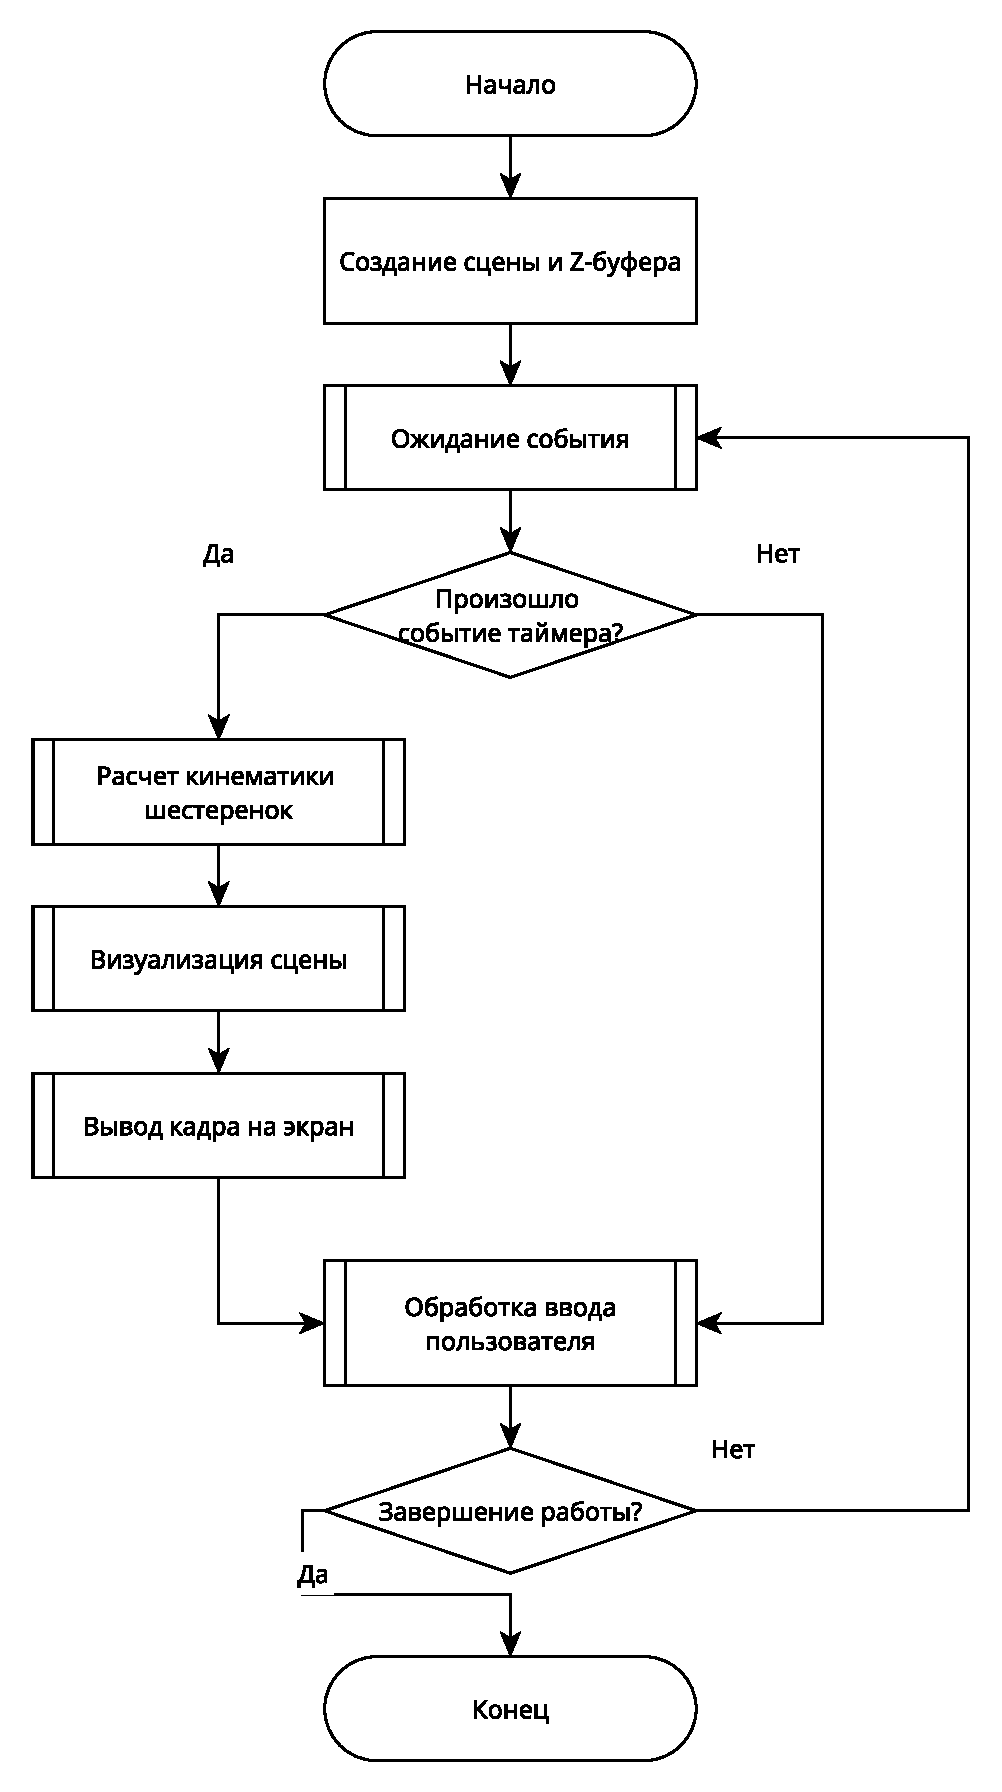
\includegraphics[width=13cm]{img/full.pdf}
	\caption{Схема алгоритма работы программы}
	\label{img:main_algo}
\end{figure}

\subsubsection{Алгоритм растеризации треугольника}

Центральным элементом графического конвейера является алгоритм растеризации треугольника с использованием Z-буфера и интерполяцией атрибутов для закраски Фонга. Схема алгоритма представлена на рисунке \ref{img:raster_algo}.

\begin{figure}[H]
	\centering
	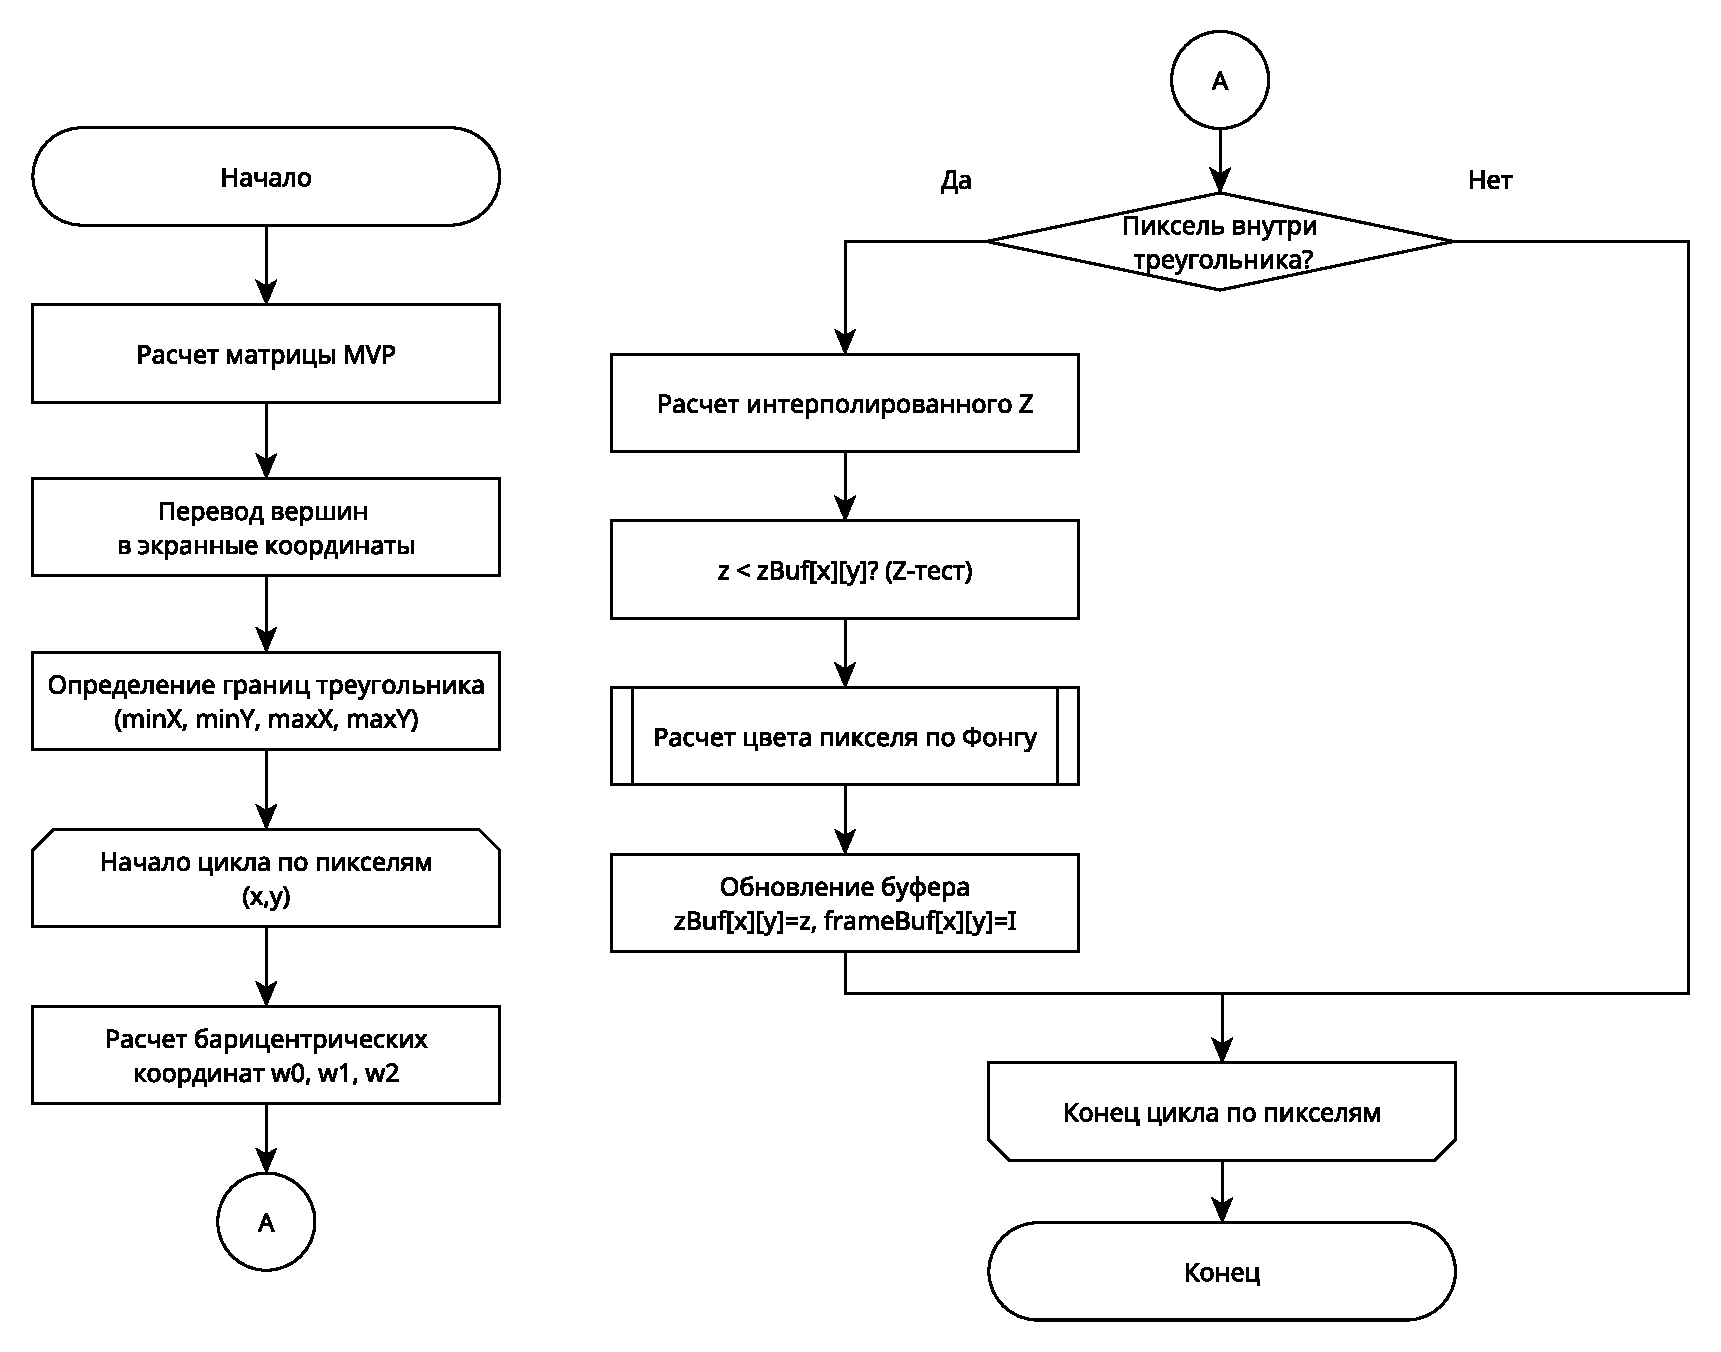
\includegraphics[width=16cm]{img/render.pdf}
	\caption{Схема алгоритма растеризации треугольника}
	\label{img:raster_algo}
\end{figure}

\subsubsection{Алгоритм расчета кинематики}

Для определения скоростей вращения всех шестеренок в механизме используется алгоритм обхода графа в ширину (BFS). Схема алгоритма представлена на рисунках~\ref{img:kinematics_algo1} и~\ref{img:kinematics_algo2}.

\begin{figure}[H]
	\centering
	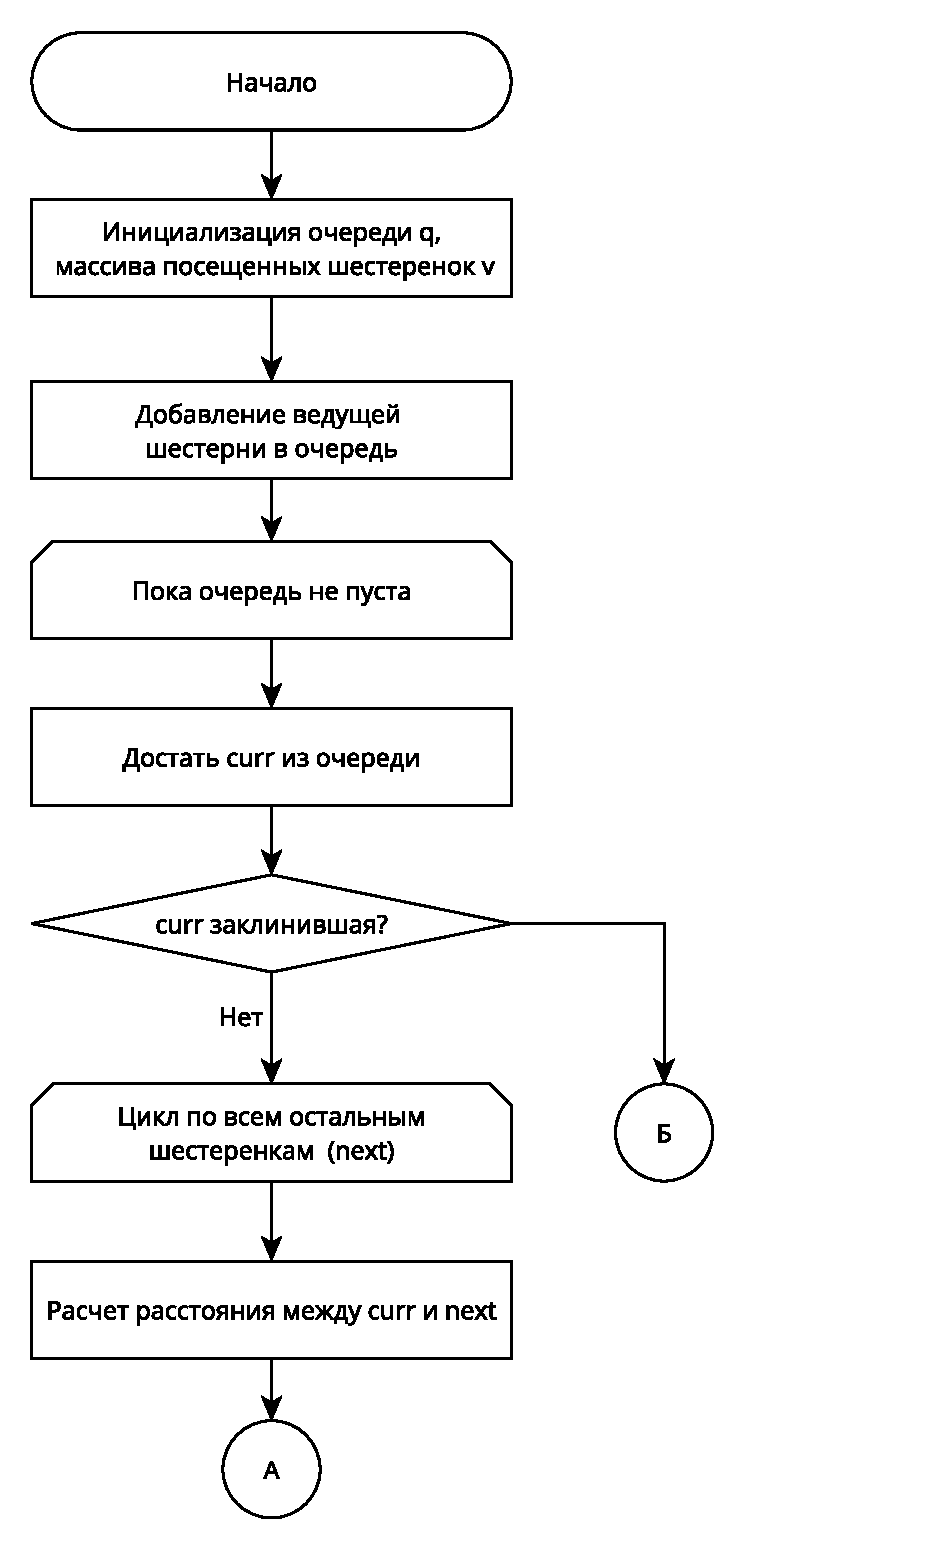
\includegraphics[width=13cm]{img/gears1.pdf}
	\caption{Схема алгоритма расчета кинематики 1}
	\label{img:kinematics_algo1}
\end{figure}
\begin{figure}[H]
	\centering
	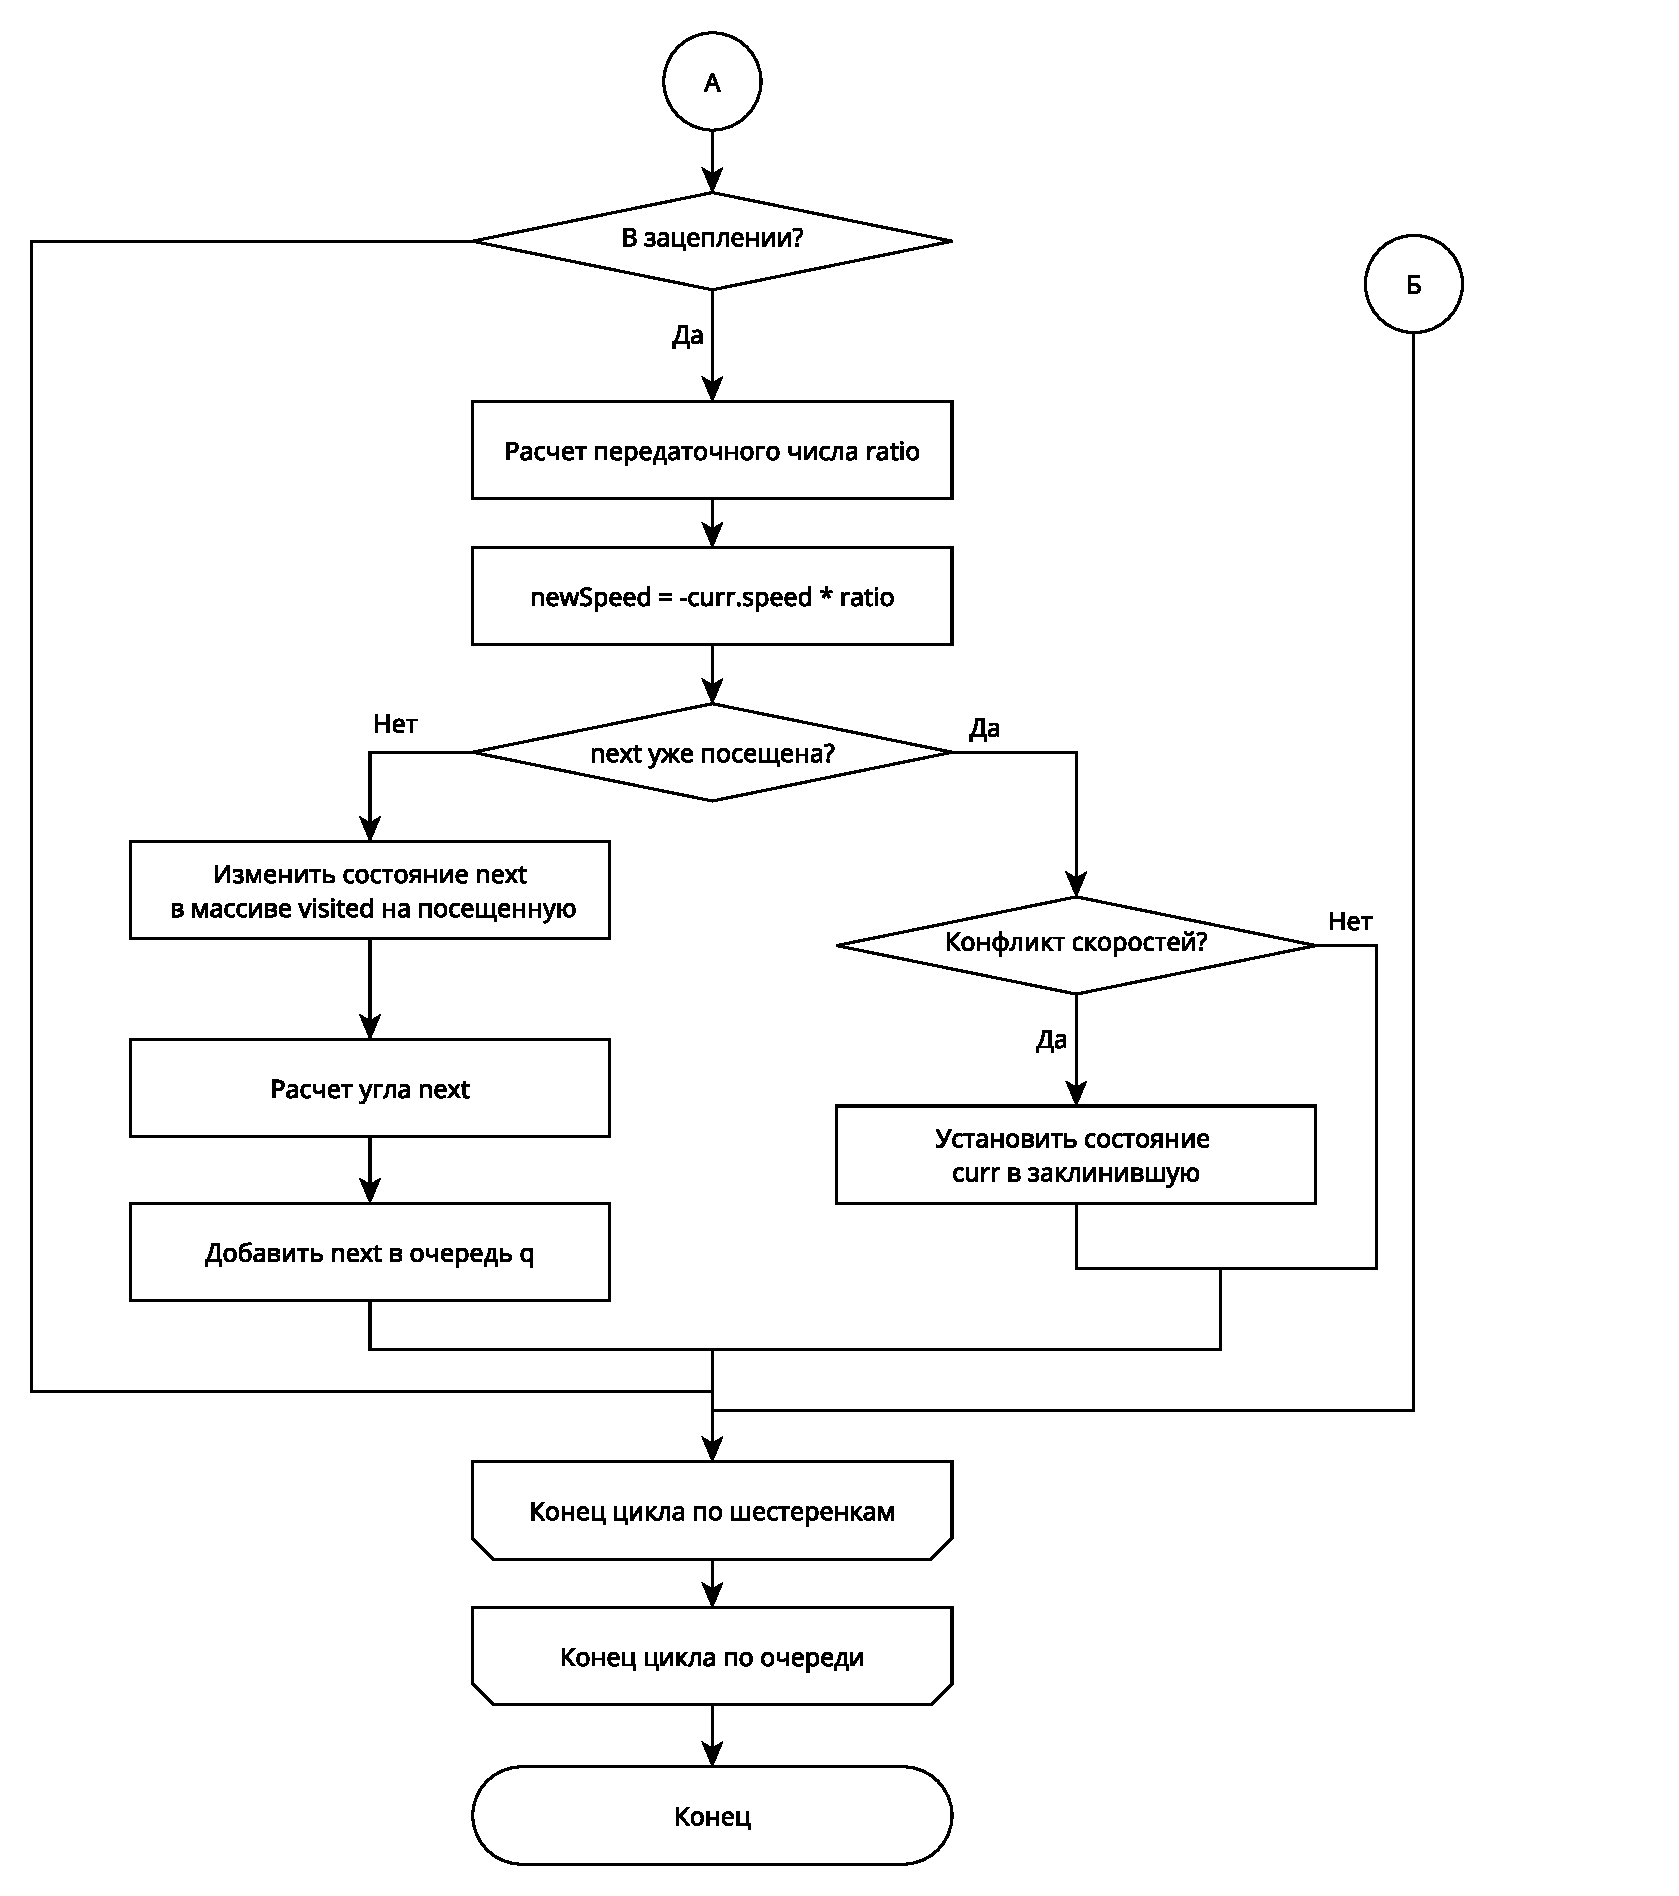
\includegraphics[width=17cm]{img/gears2.pdf}
	\caption{Схема алгоритма расчета кинематики 2}
	\label{img:kinematics_algo2}
\end{figure}


\subsection*{Вывод}

В данном разделе были сформулированы требования к программному обеспечению, включающие функциональные возможности визуализации и управления сценой. Описаны основные алгоритмы визуализации и расчета кинематики.
